\section{Linear regression}

The goal of regression is to approximate a function $f(\mathbf{x})$ that maps input $\mathbf{x}$ to a continuous output $t$ from a dataset $\mathcal{D}$: 
\[\mathcal{D}=\left\{ \left\langle \mathbf{x},t \right\rangle \right\} \implies t=f(\mathbf{x})\]
To perform regression, we assume the existence of a function capable of performing this mapping.

In linear regression, the function $f(\cdot)$ is modeled using linear functions. 
This choice is motivated by several factors:
\begin{itemize}
    \item Linear models are easily interpretable, making them suitable for explanation.
    \item Linear regression problems can be solved analytically, allowing for efficient computation.
    \item Linear functions can be extended to model nonlinear relationships.
    \item More sophisticated methods often build upon or incorporate elements of linear regression.
\end{itemize}

The key components of constructing a linear regression problem include:
\begin{itemize}
    \item \textit{Hypothesis space}: the mapping function can be defined as: 
        \[y(\mathbf{x},\mathbf{w})=w_0+\sum_{j=1}^{D-1}w_j x_j=w_01+\sum_{j=1}^{D-1}w_j x_j=\sum_{j=0}^{D-1}w_j x_j=\mathbf{w}^T\mathbf{x}\]
        The parameter $w_0=-b$ is called bias parameter. 
        In a two-dimensional space, our hypothesis space will be the set of all points in the plane $(w_0,w_1)$. 
        The coordinates of each point will correspond to a line in the $\left( \mathbf{x}, y \right)$ space.
    \item \textit{Loss function}: we usually employ the Sum of Squared Errors: 
        \[\mathcal{L}(\mathbf{w})=\dfrac{1}{2}\sum_{n=1}^{N}{\left( y(x_n, \mathbf{w})-t_n \right)}^2=\dfrac{1}{2}\sum_{n=1}^{N}{\left( \boldsymbol{\phi}(x_n)-t_n \right)}^2=\dfrac{1}{2}\text{RSS}(\mathbf{w})=\dfrac{1}{2}\sum_{i=1}^{N}\epsilon^2_i\]
    \item \textit{Optimization}: a closed-form optimization of the Residual Sum of Squares, known as Least Squares, begins with the matrix representation of the loss function:
        \[\mathcal{L}(\mathbf{w})=\dfrac{1}{2}\text{RSS}(\mathbf{w})=\dfrac{1}{2}{\left( \mathbf{w}^T\mathbf{x}-\mathbf{t} \right)}^2\]
        To find the optimal $\mathbf{w}$, we compute the first derivative of $\text{LS}(\mathbf{w})$ and set it to zero, obtaining: 
        \[\hat{\mathbf{w}}_{\text{OLS}}=(\mathbf{x}^T\mathbf{x})^{-1}\mathbf{x}^T\mathbf{t}\]
        The inversion of the matrix can be computationally expensive, especially for large datasets, assuming the matrix is non-singular (invertible). 
        
        To mitigate this, stochastic gradient descent can be employed.
        The algorithm known as Least Mean Squares uses the following update rule:
        \[\mathbf{w}^{(n+1)}= \mathbf{w}^{(n)}-\alpha\left( \mathbf{w}^{(n)}\mathbf{x}^{(n+1)}-t^{(n+1)} \right)\mathbf{x}^{(n+1)}\]

        The same update rule can be also applied for batches of size $k$: 
        \[\mathbf{w}^{(n+1)}= \mathbf{w}^{(n)}-\dfrac{\alpha}{k}\left( \mathbf{w}^{(n)}\mathbf{x}^{(n+1)}-t^{(n+1)} \right)\mathbf{x}^{(n+1)}\]
\end{itemize}

\paragraph*{Multiple outputs}
If the regression problem involves multiple outputs, meaning that $\mathbf{t}$ is not a scalar, we can solve each regression problem independently.
The solution for the weight vectors for all outputs can be expressed as:
\[\hat{\mathbf{W}}={\left( \boldsymbol{\Phi}^T\boldsymbol{\Phi}\right)}^{-1}\boldsymbol{\Phi}^T\mathbf{T}\]
This solution can be easily decoupled for each output $k$: 
\[\hat{\mathbf{w}}_k={\left( \boldsymbol{\Phi}^T\boldsymbol{\Phi}\right)}^{-1}\boldsymbol{\Phi}^T\mathbf{t}_k\]
An advantage of this approach is that ${\left( \boldsymbol{\Phi}^T\boldsymbol{\Phi}\right)}^{-1}$ only needs to be computed once, regardless of the number of outputs.

\subsection{Basis functions}
While a linear combination of input variables may not always suffice to model data, we can still construct a regression model that is linear in its parameters. 
This can be achieved by defining a model using non-linear basis functions, expressed as:
\[y(\mathbf{x},\mathbf{w})=\mathbf{w}^T\boldsymbol{\phi}(\mathbf{x})\]
Here, the components of the vector $\boldsymbol{\phi}(\mathbf{x})$ are referred to as features.
These features allow for a more flexible representation of the input data, enabling the model to capture non-linear relationships between the input variables and the output.
\begin{example}
    Let's reconsider a set of data regarding individuals' weight and height, along with their completion times for a one-kilometer run:
    \begin{table}[H]
        \centering
        \begin{tabular}{c|c|c}
        \textbf{Height (cm)} & \textbf{Weight (kg)} & \textbf{Completion time (s)} \\ \hline
        180                  & 70                   & 180                          \\
        184                  & 80                   & 220                          \\
        174                  & 60                   & 170                         
        \end{tabular}
    \end{table}
    We can model this problem using a dummy variable and introduce the Body Mass Index (BMI) as a new feature:
    \begin{table}[H]
        \centering
        \begin{tabular}{c|c|c|c|c}
        \textbf{Dummy variable} & \textbf{Height (cm)} & \textbf{Weight (kg)} & \textbf{BMI} & \textbf{Completion time (s)} \\ \hline
        $x_0$                   & $x_1$                & $x_2$                & $x_3$        & $t$                          \\
        1                       & 180                  & 70                   & 21           & 180                          \\
        1                       & 184                  & 80                   & 23           & 220                          \\
        1                       & 174                  & 60                   & 20           & 170                         
        \end{tabular}
    \end{table}
    Here, the dummy variable $x_0$ is always initialized to one.
    Now, we have the option to retain or discard the weight and height variables, considering only the BMI values for analysis.
\end{example}
The most commonly used basis functions in regression are:
\renewcommand*{\arraystretch}{2}
\begin{table}[H]
    \centering
    \begin{tabular}{|l|c|}
    \hline
    \multicolumn{1}{|c|}{\textbf{Basis function}} & \textbf{Formula}                                                                \\ \hline
    \textit{Polynomial}                           & $\phi_j(x)=x^j$                                                                 \\ \hline
    \textit{Gaussian}                             & $\phi_j(x)=e^{-\frac{{\left( x-\mu_j \right)}^2}{2 \sigma^2}}$                  \\ \hline
    \textit{Sigmoidal}                            & $\phi_j(x)=\dfrac{1}{1+e^{\frac{\mu_j-x}{\sigma}}}$                             \\ \hline
    \end{tabular}
\end{table}
\renewcommand*{\arraystretch}{1}
\begin{figure}[H]
    \centering
    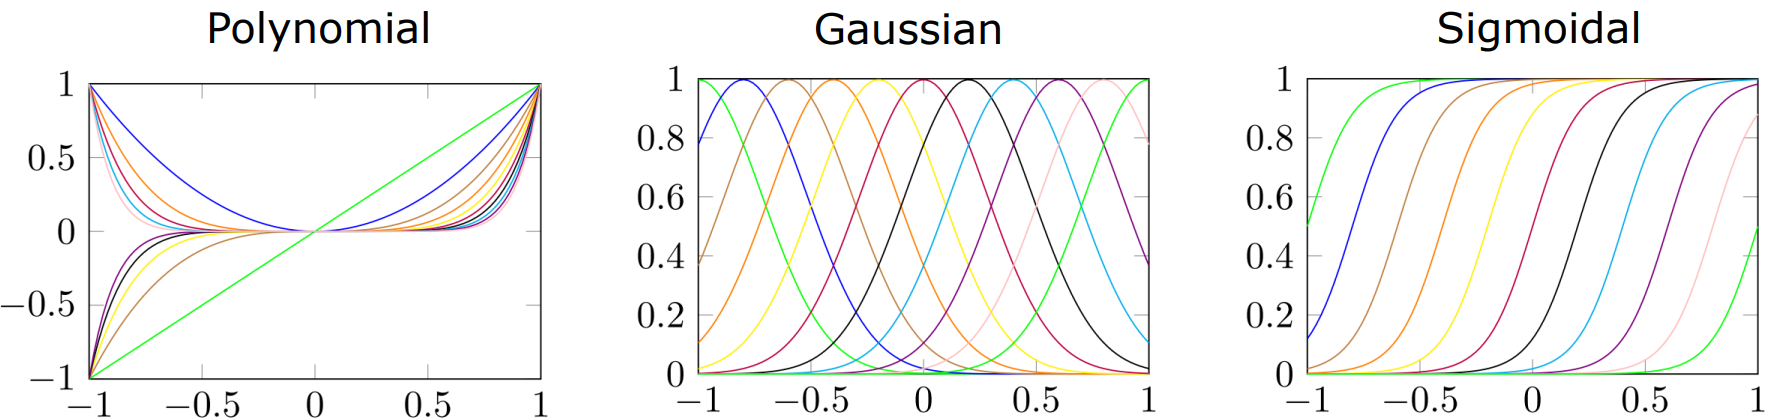
\includegraphics[width=1.00\linewidth]{images/basis.png}
    \caption{Polynomial, Gaussian, and sigmoidal basis functions}
\end{figure}
It's noteworthy that the Gaussian basis function allows for a local approximation by omitting values that are close to zero.
This approach enables capturing the relationship between the input and output in a reduced input space area.
As we move away from the mean, approaching zero, the values become negligible.

\subsection{Normalization and scaling}
Given a set of $N$ samples, $\{s_1,\dots,s_N\}$, normalization can be performed using two common methods:
\begin{itemize}
    \item \textit{Z-score} (normalization): scales the data based on the dataset's mean and standard deviation.. 
        Given the mean $\bar{s}$ and the variance $S^2=\frac{1}{N-1}\sum_{n=1}^N(s_n-\bar{s})^2$, the normalized value of a sample $s$ is calculated as:
        \[s_{\text{z-score}}=\dfrac{s-\bar{s}}{S}\]
        This method transforms the data into a distribution with a mean of 0 and a standard deviation of 1, making it useful when working with data that needs to be compared across different scales or distributions.
    \item \textit{Minmax} (feature scaling): rescales the data so that all values lie between a defined range.
        Given the minimum value $s_{\min}$ and maximum value $s_{\max}$ in the dataset, the normalized value of a sample $s$ is: 
        \[s_{\text{minmax}}=\dfrac{s-s_{\min}}{s_{\max}-s_{\min}}\]
        This method is particularly useful when the data needs to be transformed to a bounded range.
\end{itemize}
Both methods have their applications, with z-score normalization being more effective for data with outliers or differing variances, and minmax scaling suited for data that needs to be normalized to a specific range.

\subsection{Regularization}
A function can achieve a better approximation by increasing the degree of the polynomial used in the regression.
However, increasing the polynomial degree also increases the complexity of the model parameters.
To address this complexity, adjustments are needed in the loss function:
\[\mathcal{L}(\mathbf{w})=\mathcal{L}_D(\mathbf{w})+\lambda \mathcal{L}_W(\mathbf{w})\]
Here, $\mathcal{L}_D(\mathbf{w})$ represents the usual loss function, $\mathcal{L}_W(\mathbf{w})$ reflects model complexity (a hyperparameter), and $\lambda$ is the regularization coefficient.
The model complexity loss function can be: 
\begin{itemize}
    \item \textit{Ridge}, in which the loss function becomes: 
        \[\mathcal{L}_{\text{Ridge}}(\mathbf{w})=\dfrac{1}{2}\sum_{i=1}^N {\epsilon_i}^2 + \lambda\dfrac{1}{2}{\left\lVert \mathbf{w} \right\rVert}_2^2\]
        This new loss function remains quadratic with respect to $\mathbf{w}$, allowing for closed-form optimization:
        \[\hat{\mathbf{w}}_{\text{Ridge}}={\left( \lambda\mathbf{I}+\boldsymbol{\Phi}^T \boldsymbol{\Phi} \right)}^{-1}\boldsymbol{\Phi}^T\mathbf{t}\]
        The term $\lambda\mathbf{I}$ is crucial in solving the singularity problem, as it transforms a non-singular matrix into a singular one with an appropriate choice of $\lambda$.
        In particular, the eigenvalues of the $\left( \lambda\mathbf{I}+\boldsymbol{\Phi}^T \boldsymbol{\Phi} \right)$ matrix must be greater or equal than $\lambda$ since $\boldsymbol{\Phi}^T \boldsymbol{\Phi}$ is positive semidefinite. 
    \item \textit{Lasso}, in which the loss function becomes: 
        \[\mathcal{L}_{\text{Lasso}}(\mathbf{w})=\dfrac{1}{2}\sum_{i=1}^N \epsilon_i^2 + \lambda\dfrac{1}{2}{\left\lVert \mathbf{w} \right\rVert}_1\]
        In this case, closed-form optimization is not possible. 
        However, Lasso typically leads to sparse regression models: when the regularization coefficient $\lambda$ is large enough, some components of $\hat{\mathbf{w}}$ become equal to zero.
\end{itemize}

\subsection{Model evaluation}
The performance of the resulting model can be assessed through various metrics and statistical tests:
\begin{itemize}
    \item \textit{Residual Sum of Squares}: measures the discrepancy between the predicted and actual target values.
        A lower Residual Sum of Squares indicates a better fit of the model to the data.
    \item \textit{Mean Square Error}: average of the squared differences between the predicted values and the actual values. 
        It is calculated as:
        \[\text{MSE}(\mathbf{w})=\dfrac{\text{RSS}(\textbf{w})}{N}\]
        where $N$ is the number of samples. 
        Mean Square Error penalizes larger errors more heavily due to the squaring of differences.
    \item \textit{Root Mean Square Error}: square root of the Mean Square Error, giving an error metric in the same units as the target variable:
        \[\text{RMSE}(\mathbf{w})=\sqrt{\dfrac{\text{RSS}(\textbf{w})}{N}}\]
        Root Mean Square Error is often easier to interpret as it provides an error measure on the same scale as the original data.
    \item \textit{Coefficient of determination}: measures how well the model explains the variance in the target variable. 
        It is calculated as:
        \[R^2=1-\dfrac{\text{RSS}(\mathbf{w})}{\text{TSS}}\]
        Here, $\text{TSS}=\sum_{n=1}^N(\bar{t}-t_n)^2$ is the Total Sum of Squares, and $\bar{t}$ is the mean of the target values.
        An $R^2$ close to 1 indicates a good fit, while a value near 0 suggests the model performs poorly compared to a simple mean.
    \item \textit{Degrees of freedom}: represent the difference between the number of samples and the number of model parameters:
        \[\text{dfe}=N-M\]
        Here, $M$ is the number of parameters in the model.
    \item \textit{Adjusted coefficient of determination}: accounts for the number of predictors in the model and adjusts for the degrees of freedom:
        \[R^2_{\text{adj}}=1-(1-R^2)\dfrac{N-1}{\text{dfe}}\]
        This metric is useful when comparing models with different numbers of predictors, as it penalizes overfitting.
\end{itemize}

\paragraph*{Statistical tests on coeffients}
To determine the statistical significance of the model's parameters, hypothesis tests can be performed:
\begin{enumerate}
    \item \textit{Test on single coefficients}: this test examines whether each estimated weight $\hat{w}_j$ is significantly different from zero.
        The distribution for this test is given by:
        \[t_{\text{dfe}}\sim\dfrac{\hat{w}_j-w_j}{\hat{\sigma}\sqrt{v_j}}\]
        Here, $w_j$ is the true parameter, $\hat{w}_j$ is the estimated parameter, $v_j$ is the $j$-th diagonal element of $(\mathbf{x}^T\mathbf{x})^{-1}$, and $\hat{\sigma}^2$ is the unbiased estimate of the variance:
        \[\hat{\sigma}^2=\dfrac{\text{RSS}(\hat{\mathbf{w}})}{\text{dfe}}\]
        If the test shows that the coefficient is significantly different from zero, the null hypothesis (that the coefficient is zero) is rejected.
    \item \textit{Test on overall model significance}: this test assesses the significance of the overall model by comparing it to a null model (a model with no predictors).
        The test uses the Fisher-Snedecor distribution:
        \[F_\text{stat}\sim\dfrac{\text{dfe}}{M-1}\dfrac{\text{TSS}-\text{RSS}(\hat{\mathbf{w}})}{\text{RSS}(\hat{\mathbf{w}})}\]  
        If $F_\text{stat}$ is large, the null hypothesis (that all model coefficients are zero) is rejected, indicating that the model significantly improves prediction compared to a constant (mean) model.
\end{enumerate}

\subsection{Maximum Likelihood}
We can approach regression in a probabilistic framework by defining a model that maps inputs to target values probabilistically. This allows us to express uncertainty in the predictions.

Given a regression model denoted by $y(x, \mathbf{w})$, where $\mathbf{w}$ represents the unknown parameters, we assume that the observed data $\mathcal{D}$ is generated with some inherent noise.
The model provides the conditional probability of the target given the input, and we express the likelihood of the data $\mathcal{D}$ given the parameters $\mathbf{w}$ as $\Pr(\mathcal{D}\mid\mathbf{w})$. 

To estimate the parameters, we seek to find the set of parameters $\mathbf{w}$ that maximizes this likelihood.
This approach is known as Maximum Likelihood Estimation (ML), and the parameters are found by solving the following optimization problem:
\[\mathbf{w}_{\text{ML}}=\argmax_{\mathbf{w}}\Pr(\mathcal{D}\mid\mathbf{w})\]

Our probabilistic regression model can be written as:
\[t=y(\mathbf{x},\mathbf{w})+\epsilon=\mathbf{w}^T\boldsymbol{\Phi}(\mathbf{x})+\epsilon\]
Here, $y(\mathbf{x},\mathbf{w})$ is assumed to be a linear model in terms of a set of basis functions $\boldsymbol{\Phi}(\mathbf{x})$, with additive noise $\epsilon$ that follows a Gaussian distribution with zero mean and variance $\sigma^2$. 

Given a dataset $\mathcal{D}$ of $N$ samples with inputs $\mathbf{x}_n$ and targets $\mathbf{t}_n$, we express the likelihood of the data $\mathcal{D}$ given the model parameters $\mathbf{w}$ as: 
\[\Pr(\mathcal{D}\mid \mathbf{w})=\Pr(\mathbf{t}\mid\mathbf{x},\mathbf{w},\sigma^2)=\prod_{n=1}^{N}\mathcal{N}(t_n\mid\mathbf{w}^T\boldsymbol{\Phi}(\mathbf{x}_n),\sigma^2)\]
Here, $\mathcal{N}(t_n\mid\mathbf{w}^T\boldsymbol{\Phi}(\mathbf{x}_n),\sigma^2)$ represents the Gaussian distribution for each target, with mean $\mathbf{w}^T\boldsymbol{\Phi}(\mathbf{x}_n)$ and variance $\sigma^2$. 

To find the Maximum Likelihood estimate $\mathbf{w}_{\text{ML}}$, we maximize the log-likelihood, which simplifies the product into a sum:
\[\mathcal{L}(\mathbf{w})=\ln\Pr(t_n\mid \mathbf{x}_n, \mathbf{w} ,\sigma^2)=-\dfrac{N}{2}\ln(2\pi\sigma^2)-\dfrac{1}{2\sigma^2}\text{RSS}(\mathbf{w})\]
Here, $RSS(\mathbf{w})$ is the Residual Sum of Squares.

The first term, $-\frac{N}{2}\ln(2\pi\sigma^2)$, is independent of $\mathbf{w}$, so we can ignore it when maximizing the log-likelihood.
This leaves us with the second term, which is proportional to the residual sum of squares. 
Therefore, maximizing the log-likelihood is equivalent to minimizing $\text{RSS}(\mathbf{w})$. 

To find $\mathbf{w}_{\text{ML}}$, we set the gradient of $\mathcal{L}(\mathbf{w})$ with respect to $\mathbf{w}$ to zero: 
\[\dfrac{\partial \mathcal{L}(\mathbf{w})}{\partial\mathbf{w}}=0\]
Solving this yields the closed-form solution for the Maximum Likelihood estimate of $\mathbf{w}$
\[\mathbf{w}_{\text{ML}}={\left( \boldsymbol{\Phi}^T\boldsymbol{\Phi} \right)}^{-1}\boldsymbol{\Phi}^T\mathbf{t}\]
This result matches the solution for the Ordinary Least Squares method, showing that the Maximum Likelihood estimate under the assumption of Gaussian noise is equivalent to minimizing the squared error.
The Maximum Likelihood estimate $\mathbf{w}_{\text{ML}}$ has the smallest variance among unbiased linear estimators, according to the Gauss-Markov theorem.

\subsection{Bayesian linear regression}
Bayesian linear regression offers a probabilistic framework for modeling linear relationships by incorporating uncertainty about the model parameters, unlike traditional methods that provide only point estimates. 
In this approach, we treat the model parameters as random variables and update our beliefs about them as more data becomes available.
The process is outlined in the following steps:
\begin{enumerate}
    \item \textit{Formulation of a probabilistic model}: initially, we express our prior knowledge about the model parameters probabilistically, defining a prior distribution that encapsulates assumptions about these parameters before observing any data. 
        This prior reflects what we know or assume about the parameter values based on domain expertise or past experience.
        Assuming a Gaussian likelihood function allows the use of a conjugate Gaussian prior, which simplifies the Bayesian updating process. 
        The prior is typically modeled as:
        \[\Pr(\mathbf{w})=\mathcal{N}(\mathbf{w}\mid\mathbf{w}_0,\mathbf{S}_0)\]
        Here, $\mathbf{w}_0$ is the prior mean, and $\mathbf{S}_0$ is the prior covariance matrix.
    \item \textit{Data observation}: as we collect data, we obtain a likelihood function that measures the probability of observing the data given particular values of the model parameters.
        After observing the data, the posterior remains Gaussian:
        \[\begin{cases}
            \Pr(\mathbf{w}\mid\mathbf{t},\boldsymbol{\Phi},\sigma^2)=\mathcal{N}(\mathbf{w}\mid\mathbf{w}_N,\mathbf{S}_N) \\
            \mathbf{w}_N=\mathbf{S}_N\left(\mathbf{S}_0^{-1}\mathbf{w}_0+\dfrac{\boldsymbol{\Phi}^T\mathbf{t}}{\sigma^2}\right) \\
            \mathbf{S}_N^{-1}=\mathbf{S}_0^{-1}+\dfrac{\boldsymbol{\Phi}^T\boldsymbol{\Phi}}{\sigma^2}
        \end{cases}\]
        Here, $\mathbf{w}_N$ is the posterior mean, and $\mathbf{S}_N$ is the posterior covariance matrix.
    \item \textit{Posterior distribution calculation}: after observing the data, we use Bayes' theorem to compute the posterior distribution, which combines the prior distribution with the likelihood of the data.
        In Bayesian linear regression, the posterior distribution is computed by combining the prior with the likelihood of the parameters given the observed data:
        \[\Pr(\mathbf{w}\mid\mathcal{D})=\dfrac{\Pr(\mathcal{D}\mid\mathbf{w})\Pr(\mathbf{w})}{\Pr(\mathcal{D})}\]
        Here, $\Pr(\mathbf{w})$ is the prior distribution over the parameters $\mathbf{w}$, $\Pr(\mathcal{D}\mid\mathbf{w})$ is the likelihood of the data given the parameters, and $\Pr(\mathcal{D})$ is the marginal likelihood.
        The prior mean could be: 
        \begin{itemize}
            \item \textit{Infinitely broad}: if the prior is uninformative, the covariance matrix $\mathbf{S}_0$ ends to infinity, leading to:
                \[\lim_{\mathbf{S}_0\rightarrow\infty}\mathbf{w}_N={\left( \boldsymbol{\Phi}^T\boldsymbol{\Phi} \right)}^{-1}\boldsymbol{\Phi}^T\mathbf{t} \qquad \lim_{\mathbf{S}_0\rightarrow\infty}\mathbf{S}_N^{-1}=\dfrac{\boldsymbol{\Phi}^T\boldsymbol{\Phi}}{\sigma^2}\]
                This reduces the Bayesian solution to the Ordinary Least Squares solution, and the MAP estimate becomes equivalent to the Maximum Likelihood estimate. 
                The variance $\sigma^2$ can be estimated as:
                \[\sigma^2=\dfrac{1}{N-M}\sum_{n=1}^{N}{\left( t_n-\hat{\mathbf{w}}^T\boldsymbol(\phi)(\mathbf{x}_n) \right)}^2\]
            \item \textit{Not infinitely broad}: in cases where the prior is informative (e.g., $\mathbf{w}_0=0$, $\mathbf{S}_0=\tau^2\mathbf{I}$), the posterior can be expressed as:
                \[\ln\Pr(\mathbf{w}\mid\mathbf{t})=-\dfrac{1}{2}\sum_{i=1}^{N}{\left(t_i-\mathbf{w}^T\boldsymbol{\phi}(\mathbf{x}_i)\right)}^2-\dfrac{\sigma^2}{2\tau^2}{\left\lVert \mathbf{w}\right\rVert}_2^2 \]
                The Maximum A Posteriori estimate coincides with the solution to Ridge regression, where the regularization parameter $\lambda$ is related to the prior by $\lambda=\frac{\sigma^2}{\tau^2}$.
        \end{itemize}
    \item \textit{Prediction and decision making}: to make predictions, we use the posterior distribution by averaging over all possible parameter values weighted by their posterior probabilities. 
        This allows for uncertainty in the predictions and enables decisions that minimize expected loss.
        Under Gaussian assumptions, the predictive distribution remains Gaussian with mean and variance:
    \[\mu_N(\mathbf{x})=\boldsymbol{\phi}(\mathbf{x})^T\mathbf{w}_N \qquad\sigma_N^2(\mathbf{x})=\sigma^2+\boldsymbol{\phi}{(\mathbf{x})}^T\mathbf{S}_N\boldsymbol{\phi}(\mathbf{x})\]
\end{enumerate}
As the number of data points $N$ increases, the uncertainty in the parameters (captured by the second term) diminishes, leaving only the variance of the noise $\sigma^2$. 

\subsection{Challenges and limitations}
Modeling presents challenges in ensuring our model effectively represents a wide range of plausible functions while maintaining informative priors without overly spreading out probabilities or assigning negligible values.

On the computational side, limitations arise with analytical integration, particularly in cases involving non-conjugate priors and complex models. 
Approaches like Gaussian approximation, Monte Carlo integration, and variational approximation become necessary for addressing these complexities and achieving accurate results.

Linear models with fixed basis functions offer several benefits:
\begin{itemize}
    \item They permit closed-form solutions, facilitating efficient computation.
    \item They lend themselves to tractable Bayesian treatment, enabling principled uncertainty quantification.
    \item They can capture non-linear relationships by employing appropriate basis functions.
\end{itemize}
However, these models also come with several drawbacks:
\begin{itemize}
    \item Basis functions remain static and non-adaptive to variations in the training data.
    \item These models are susceptible to the curse of dimensionality, particularly when dealing with high-dimensional feature spaces.
\end{itemize}